% !TEX root = ../Dokumentation.tex
\subsection{Energieversorgung}

\textbf{Funktionsbeschrieb}\\[0.2cm]
Das autonome Entsorgungsfahrzeug muss mit Energie versorgt werden. Dazu werden Akkumulatoren eingesetzt, welche das Gerät während dem gesamten Einsatz mit Strom versorgen. 
\\[0.2cm]
\textbf{Komponentenbeschrieb}
Um Störungen, die z.B durch den erhöten Anlaufstrom der Motoren verursacht werden könnten zu vermeiden, werden die intelligenten Systeme (Microcontroller, Mini-Computer,etc.) möglichst getrennt von den Motoren gespiesen. Dazu werden zwei Lithium-Polymer-Akkumulatoren mit einer voraussichtlichen Spannung von 11.1 und 7.4 Volt verwendet die galvanisch getrennt sind.
Der 11.1 Volt Akkumulator wird die Versorgung der Motoren gewährleisten und eine Kapazität von 2000-2400 mAh aufweisen. Für die empfindlicheren Systeme wird der 7.4 Volt LiPo zuständig sein, der eine Kapazität von 500-1000 mAh besitzt.
Die genaue Evaluation der Kapazitäten ist noch nicht abgeschlossen und bezieht sich lediglich auf die Resultate der Rechnungen, welche im Verlauf des Kapitels noch beschrieben werden.
\begin{figure}[H]
\centering
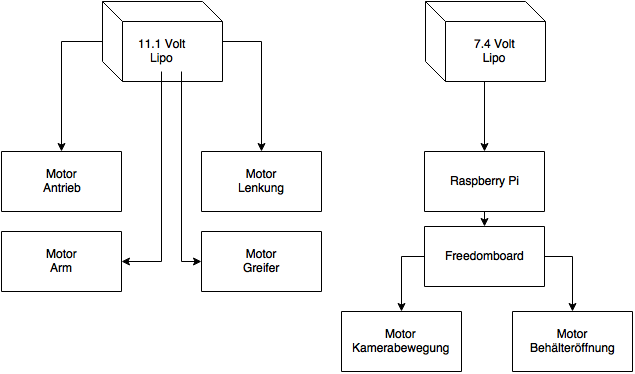
\includegraphics[width=0.8\textwidth]{03_Loesungskonzept/pictures/speisung.png}
\caption{Aufteilung der Akkumulatoren}	
\end{figure}\flushleft
\textbf{Begründung}\\[0.2cm]
Die Entscheidung wird damit begründet, dass Lithium-Polymer-Akkumulatoren in einem vielfältigen Sortiment erhältlich sind und damit eine grosse Flexibilität bei der Auswahl ermöglichen. Somit würde sich auch die Suche nach einem Ersatz bei allfälligen Änderungen vereinfachen. Ausserdem weisen LiPos, im Vergleich zu anderen Akkumulatoren eine wesentlich kompaktere Bauform auf, was entscheidend für die Auswahl war. \\[0.2cm]
\textbf{Berechnungen}\\[0.2cm]
Da die Wahl der Servomotoren für die Lenkung und den Greiferarm noch nicht definitiv feststeht, werden für die Berechnung Motoren genommen, die den Anforderungen am nächsten kommen.\\
Leistungsberechnungen:
\begin{itemize}
\item Servomotor für die Lenkung:
\[
P=2\cdot \pi\cdot N\cdot M \to 2\cdot \pi\cdot 0.92\frac{U}{sec}\cdot 0.65Nm = 3.76W
\]
\item Servomotoren für Kamerabewegung, Greifer und Behälteröffnung:
\[
P=2\cdot \pi\cdot N\cdot M \to 2\cdot \pi\cdot 0.72\frac{U}{sec}\cdot 0.18Nm = 0.81W
\]
\item Servomotor für den Greiferarm:
\[
P=2\cdot \pi\cdot N\cdot M \to 2\cdot \pi\cdot 1.14\frac{U}{sec}\cdot 0.32Nm = 2.5W
\]
\item DC-Motor für den Antrieb:
\[
P=2\cdot \pi\cdot N\cdot M \to 2\cdot \pi\cdot 5.258\frac{U}{sec}\cdot 2.23Nm = 73.98W
\]
\end{itemize}
Kapazitätenberechnungen:
\begin{itemize}
\item DC-Motor für den Antrieb:
\[
\frac{P\cdot t}{U} \to \frac{73.98W\cdot0.25h}{12V}= 1.54 Ah
\]
\item Servomotor für die Lenkung:
\[
\frac{P\cdot t}{U} \to \frac{3.76W\cdot0.25h}{4.8V}= 0.19 Ah
\]
\item Servomotor für den Greiferarm:
\[
\frac{P\cdot t}{U} \to \frac{2.5W\cdot0.25h}{4.8V}= 0.13 Ah
\]
\item Servomotoren für Kamerabewegung, Greifer und Behälteröffnung:
\[
\frac{P\cdot t}{U} \to \frac{0.81W\cdot0.25h}{4.8V}= 0.04 Ah
\]
\item Mini-Computer:
\[
I\cdot t \to 2A+0.25h = 0.5 Ah
\]
\item Benötigte Kapazität für den 11.1 Volt Akkumulator:
\[
1.54Ah+0.19Ah+0.13Ah+0.04Ah = 1.9Ah
\]
\item Benötigte Kapazität für den 7.4 Volt Akkumulator:
\[
0.5Ah
\]
\end{itemize}
